% Auto-generated by experiments/build_coherence_heatmap.py
\begin{figure}[!htb]
\centering
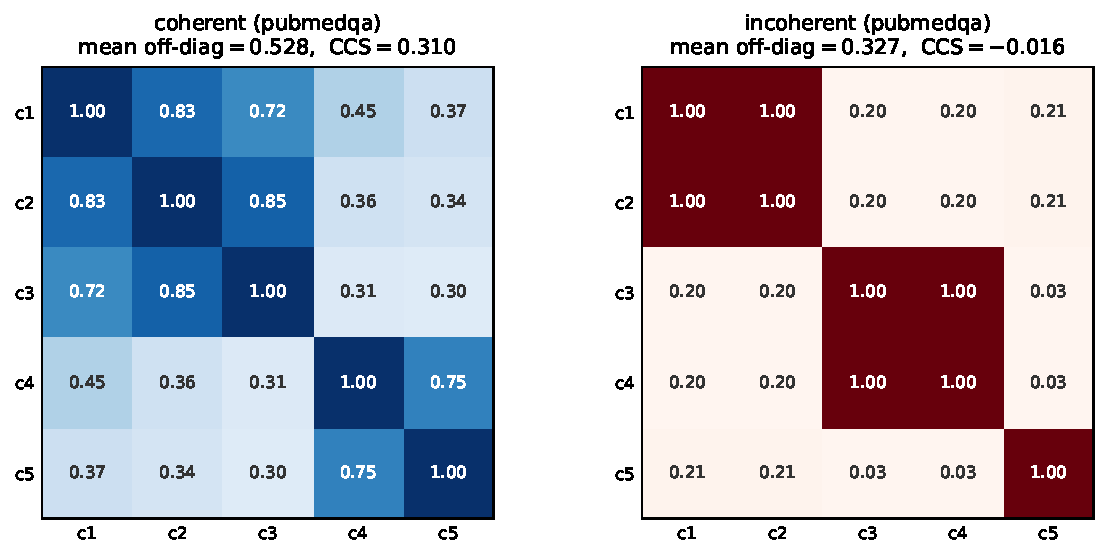
\includegraphics[width=\linewidth]{figures/coherence_heatmap.pdf}
\caption{\textbf{Coherent vs incoherent retrieval sets, visualized.}
Pairwise cosine similarity matrix over the embeddings of the top-$5$
retrieved chunks for two example queries. Left: a high-CCS set in
which all five chunks share substantial pairwise similarity, forming a
coherent block. Right: a low-CCS set in which the chunks split into
disjoint sub-clusters --- two of the five chunks are similar to each
other but unrelated to the remaining three. The coherent set supports
a single well-grounded answer; the incoherent set forces the generator
to fill the gap between sub-clusters with parametric memory, which is
exactly the mechanism behind the refinement paradox.}
\label{fig:coherence_heatmap}
\end{figure}
